\begingroup
\ArithmeticHead{237}{R}{\scriptsize AUS SCHUMACHERS GAUSSIANA.}
\SourceLeaf{244b}
\pdfbookmark[1]{[3.] Gauss an Bessel, 3. September 1805}{x1-correspondence-3}
\NumberedItem{3}
\begin{center}\textsc{Gauss} an \textsc{Bessel}.\quad Braunschweig, den 3. September 1805.\end{center}
\HistoricCitation{[Briefwechsel zwischen \textsc{Gauss} und \textsc{Bessel}, Leipzig 1880, S. 10—14.]}
\noindent .\quad .\quad .\quad .\quad .\quad .\quad Sie haben mir gütigst erlaubt, zuweilen bei meinen astronomischen Arbeiten Ihre bereitwillige Gefälligkeit in Anspruch zu nehmen: schon einmal haben Sie die Freundschaft gehabt, eine beschwerliche Rechnung für mich zu übernehmen, und schon wieder bin ich so frei, Ihnen eine neue zuzumuthen. Ich habe mich schon seit einiger Zeit mit Perturbationsrechnungen beschäftigt, wo ich hauptsächlich zum Behuf von Planeten wie Pallas und Juno, die eine starke Excentricität oder Neigung haben, mir eine eigne Methode ausgedacht habe, bei der allerdings viel, sehr viel Arbeit ist, der aber dies nicht zum Vorwurf gereichen kann, da, meinem Urtheile nach, alle bisherigen Methoden in einem solchen Falle ganz unzulänglich sind. Etwas Charakteristisches bei dieser Methode ist es, dass die Entwickelung
\clearpage
\ArithmeticHead{238}{L}{ANALYSIS. BRIEFWECHSEL.}
\SourceLeaf{245}
\noindent der Coefficienten eines solchen Ausdruckes
\[
\begin{aligned}
(aa+a'a'-2aa'\cos\varphi)^{-\frac12}
&=\tfrac12 A^0+A'\cos\varphi+A''\cos2\varphi\\
&\qquad{}+A'''\cos3\varphi\ \text{etc.}
\end{aligned}
\]
\noindent nicht wie bei den bisher üblichen Methoden bloss für Einen bestimmten Werth von $a,a'$ sondern für eine grosse Menge verschiedener Werthe erforderlich werden. Z. B. Bei einer Rechnung, die ich für die Ceres\textsuperscript{[*)]} unternommen habe, habe ich 50 gebraucht; bei Pallas und Juno werden noch mehrere erforderlich sein.

\par\indent Nun bin ich im Besitz von besonderen, zum Theil auf ganz heterogen scheinende Untersuchungen gegründeten Kunstgriffen, jene Coefficienten mit sehr grosser Geschwindigkeit zu bestimmen. Indess macht die grosse Menge doch immer die Arbeit beschwerlich und ich habe es daher [vor], zumal da für jeden Planeten die Arbeit mehrere Male (mit den successive verbesserten Elementen) wird gemacht werden müssen, ein für allemal eine Tabelle zu berechnen, mit deren Hülfe man dann \textls[120]{mit sehr geringer Arbeit} die gesuchten Coefficienten angeben könne, und bei dieser Gelegenheit bin ich so unbescheiden, mir in Etwas Ihre Unterstützung auszubitten.

\par\indent Begreiflich darf die Tafel nicht $A^0,A'$ etc. selbst angeben, weil sie sonst doppelte Eingänge haben müsste. Hingegen zu $aA^0,aA',aA''$ etc. oder $a'A^0,a'A',a'A''$ etc. braucht man nur Einen Eingang, da diese Grössen bloss Functionen von $\dfrac a{a'}$ sind. Es ist nicht schwer, $\dfrac a{a'}=f$ gesetzt (in der Vorauss[etzung] $a<a'$), folgende Reihen zu entwickeln:
\[
\begin{aligned}
\tfrac12 a'A^0&=1+\frac14ff+\frac14.\frac9{16}f^4+\frac14.\frac9{16}.\frac{25}{36}f^6+\text{etc.}\\[.7em]
&=1+\frac12.\frac12ff+\frac{1.3}{2.4}.\frac{1.3}{2.4}f^4\\[.5em]
&\qquad{}+\frac{1.3.5}{2.4.6}.\frac{1.3.5}{2.4.6}f^6+\text{etc.}\\[.7em]
\tfrac12 a'A'&=\frac12 f\Bigl(1+\frac12.\frac34ff+\frac{1.3}{2.4}.\frac{3.5}{4.6}f^4\\[.5em]
&\qquad{}+\frac{1.3.5}{2.4.6}.\frac{3.5.7}{4.6.8}f^6+\text{etc.}\Bigr)\\[.7em]
\tfrac12 a'A''&=\frac12.\frac34ff\Bigl(1+\frac12.\frac56ff+\frac{1.3}{2.4}.\frac{5.7}{6.8}f^4\\[.5em]
&\qquad{}+\frac{1.3.5}{2.4.6}.\frac{5.7.9}{6.8.10}f^6+\text{etc.}\Bigr)
\end{aligned}
\]
\centerline{etc.}
\par\vfill\noindent\rule{.25\linewidth}{.4pt}\par\smallskip
\begingroup\footnotesize\noindent [*) In der Handschrift steht hier und im folgenden auch für Pallas und Juno das entsprechende Zeichen.]\par\endgroup
\clearpage
\ArithmeticHead{239}{R}{GAUSS AN BESSEL.}
\SourceLeaf{246}
\noindent Ferner ist bekannt, dass folgende Gleichungen Statt finden:
\[
\begin{aligned}
A^0-2\left(f+\frac1f\right)A'+3A''&=0\\[.6em]
3A'-4\left(f+\frac1f\right)A''+5A'''&=0\\[.6em]
5A''-6\left(f+\frac1f\right)A'''+7A^{\mathrm{IV}}&=0\ \text{etc.}
\end{aligned}
\]
\noindent Gewöhnlich berechnet man $A^0$ und $A'$ aus obigen Reihen und dann daraus vermittelst eben gedachter Formeln $A''$, $A'''$, $A^{\mathrm{IV}}$ etc. Allein diess Verfahren ist zu meinem Zwecke unbrauchbar, »denn wenn $A^0$ oder $A'$ nur etwas weniges\newline
»fehlerhaft sind z. B. nur um 1 in der $7^{\mathrm{ten}}$ Decimale, so werden die daraus\newline
»bei $A''$, $A'''$ etc. entspringenden Fehler immer grösser, beinahe in Geometrischer\newline
»Progression, diess ist desto beträchtlicher, je kleiner $f$ ist, und man kann für\newline
»die entfernteren Coefficienten, z. B. für $A^{\mathrm X}$, welcher bei Pallas wol nöthig\newline
»sein kann, \textls[120]{ganz und gar falsche} Werthe erhalten.« Diese Bemerkung ist meines Wissens noch nicht gemacht, aber von Wichtigkeit. Ich habe daher auf eine ganz andere Methode gedacht, wo ich die Logarithmen selbst von $A^{\mathrm X}$ bis auf die $6^{\mathrm{te}}$ Ziffer mit den gewöhnlichen Logarithmen Tafeln genau erhalte. Ehe ich diese erkläre, bemerke ich noch, dass ich nicht $a'A^0,a'A',a'A'',a'A'''$ etc. in meiner Tafel ansetze. 1) sind mir zu meinen Zwecken die Logarithmen angemessener, 2) würden die Logarithmen von diesen Grössen zu stark sich ändern und das Interpoliren zu beschwerlich machen. Ich habe es vielmehr am dienlichsten gefunden, die Logarithmen von
\[
\begin{aligned}
A^0\surd(a'a'-aa)&=B^0\\[.5em]
\frac{A'}f\surd(a'a'-aa)&=B'\\[.5em]
\frac{A''}{ff}\surd(a'a'-aa)&=B''\\[.5em]
\frac{A'''}{f^3}\surd(a'a'-aa)&=B'''\ \text{etc.}
\end{aligned}
\]
\noindent anzusetzen, und zum Argumente der Tafel den Winkel zu nehmen $(=W)$, dessen Tangente $\dfrac a{a'}=f$ ist. Die Tafel selbst soll von Minute zu Minute gehen und zwar fürs erste so weit als für die drei neuen Planeten zureicht, nemlich von $17^0$ bis $35^0$. Natürlich aber berechne ich die Tafel nicht un-
\clearpage
\ArithmeticHead{240}{L}{ANALYSIS. BRIEFWECHSEL.}
\SourceLeaf{247}
\noindent mittelbar von Minute zu Minute, sondern Anfangs nur von $32'$ zu $32'$ und weiterhin von $16'$ zu $16'$ (nämlich von $33^0$ an), das übrige findet sich dann eben so genau durch eigne Interpolations Methoden.

\par\indent Ich habe demnach nach meinem Zuschnitte nöthig\newline
die Logarithmen von $B^0,B',B''\ldots B^{\mathrm X}$ für die Werte von $W$
\[
\begin{gathered}
16^0\,20',\quad16^0\,52',\quad17^0\,24'\ .\ .\ .\ .\ .\ 32^0\,20',\\
32^0\,36',\quad32^0\,52'\ .\ .\ .\ .\ .\ 36^0\,4'
\end{gathered}
\]
\noindent zusammen für 45 Werthe. Nun nehme ich über mich selbst
\begin{list}{}{\leftmargin=3em\itemsep=0pt\parsep=0pt\topsep=.5em}
\item[1)] das ganze Interpolationsgeschäft
\item[2)] die ganze Rechnung für die 17 letzten Werthe
\item[3)] die Berechnung von $B^0$ und $B'$ für die 28 ersten
\end{list}
\noindent und ersuche Sie zu übernehmen die Berechnung der übrigen Coefficienten für die 28 ersten Werthe, von $16^0\,20'$ bis $30^0\,44'$ inclus[ive].

\par\indent Meine Berechnungsmethode ist nun folgende.

\par\indent Ich setze
\newcommand{\BesselMoon}{\mathord{\vcenter{\hbox{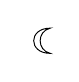
\begin{tikzpicture}[x=1cm,y=1cm]\draw[line width=.35pt] (.12,.16) .. controls (-.16,.16) and (-.16,-.16) .. (.12,-.16) .. controls (-.05,-.12) and (-.05,.12) .. cycle;\end{tikzpicture}}}}}
\[
\left.\begin{aligned}
B^0&=2N^0B'(1+ff)\\
3B'&=4N'B''(1+ff)\\
5B''&=6N''B'''(1+ff)\\
7B'''&=8N'''B^{\mathrm{IV}}(1+ff)\\
&\qquad\text{etc.}
\end{aligned}\right\}\ (\odot)
\]
\noindent dadurch wird
\[
\left.\begin{aligned}
N^0&=1-\frac98\left(\frac f{1+ff}\right)^2\frac1{N'}\\[.6em]
N'&=1-\frac{25}{24}\left(\frac f{1+ff}\right)^2\frac1{N''}\\[.6em]
N''&=1-\frac{49}{48}\left(\frac f{1+ff}\right)^2\frac1{N'''}\\
&\qquad\text{etc.}
\end{aligned}\right\}\ (\BesselMoon)
\]
\par\indent Man kann vermittelst dieser Formel $N^0,N',N''$ etc. durch continuirliche Brüche leicht darstellen; allein folgender Ausdruck, auf den ich gekommen bin, ist noch viel brauchbarer:
\clearpage
\ArithmeticHead{241}{R}{GAUSS AN BESSEL.}
\SourceLeaf{248}
\[
\frac1{N^n}=\cfrac{1+ff}{1-\cfrac{\frac1{(2n+3)^2-1}ff}{1-\cfrac{\frac{(2n+3)^2}{(2n+5)^2-1}ff}{1-\cfrac{\frac9{(2n+7)^2-1}ff}{1-\cfrac{\frac{(2n+5)^2}{(2n+9)^2-1}ff}{1-\cfrac{\frac{25}{(2n+11)^2-1}ff}{1-\cfrac{\frac{(2n+7)^2}{(2n+13)^2-1}ff}{1-\text{etc.}}}}}}}}
\]
\noindent wo das alternirende Gesetz offenbar genug ist. Folglich wird
\[
(1+ff)N^{\mathrm X}=1-\cfrac{\frac1{528}ff}{1-\cfrac{\frac{529}{624}ff}{1-\cfrac{\frac9{728}ff}{1-\cfrac{\frac{625}{840}ff}{1-\cfrac{\frac{\mathbf{25}}{\mathbf{960}}\mathbf{ff}}{1-\cfrac{\frac{\mathbf{729}}{\mathbf{1088}}\mathbf{ff}}{1-\cfrac{\frac{\mathbf{49}}{\mathbf{1224}}\mathbf{ff}}{1-\text{etc.}}}}}}}}
\]
\noindent Sie können hier ohne Bedenken die rothen\textsuperscript{[*)]} Grössen ganz vernachlässigen, da sie kaum eine Einheit in der $7^{\mathrm{ten}}$ Decimale machen können. Ich habe bei den letzten Werthen von $W$ noch ein Paar mehr genommen.

\par\indent Nun, vermittelst dieser Formel berechne ich $\log N^{\mathrm X}$, daraus nach der Formel $(\BesselMoon)$ rückwerts $N^{\mathrm{IX}},N^{\mathrm{VIII}}\ldots N^0$, welche alle bis auf die $7^{\mathrm{te}}$ Decimale zuverlässig werden. Ferner berechne ich nach einer eigenthümlichen äusserst bequemen Methode, die ich Ihnen in der Folge gern auch mittheile, $\log B^0$ und $\log B'$ (letztern bloss der Controle wegen), und Endlich aus $\log B^0$ und den Log[arithmen] von $N^0,N'\ldots N^{\mathrm{IX}}$ vermittelst der Formeln $(\odot)$ die Log[a-
\par\vfill\noindent\rule{.25\linewidth}{.4pt}\par\smallskip
\begingroup\footnotesize\noindent [*) Die in der Handschrift mit roter Tinte geschriebenen Zahlen und Buchstaben sind hier fett gedruckt.]\par\endgroup
\smallskip\noindent\small X 1.\hfill31\normalsize
\clearpage
\ArithmeticHead{242}{L}{ANALYSIS. BRIEFWECHSEL.}
\SourceLeaf{249}
\noindent rithmen] von $B',B''\ldots B^{\mathrm X}$; der Logarithmus von $B'$ darf von dem auf dem andern Wege gefundenen nur höchstens um 2 in der $7^{\mathrm{ten}}$ Stelle differiren, in welchem Falle ich, um $B''$ daraus abzuleiten, gewöhnlich das Mittel nehme; ist der Unterschied 1, so ziehe ich den letztgenannten vor, ist er grösser, so liegt gewiss entweder in der einen oder der anderen Rechnung ein Fehler.
\par\noindent .\quad .\quad .\quad .\quad .
\clearpage
\endgroup
